
\subsection{Groups}

Two ways to define groups
\begin{itemize}
    \item concrete: group = symmetries of an object $X$. Here a symmetry is a bijection $X \to X$ with inverse that preserves ``structure'' (topology, order, binary operation, $\ldots$)
\end{itemize}

\begin{example}
    The rectangle has 4 symmetries. \\
    The icossahedron has $20 \times 3$ symmetries since after fixing the first face there are 3 possible rotations. \\
    Vector space $\bR^k$: $n \times n$ matrices with $\det \neq 0$, denoted $GL_n(K)$
\end{example}

\begin{itemize}
    \item abstract definition: \\
    \begin{definition}
        A group is a set $G$ with a binary operation $G \times G \to G$ by $(a,b) \mapsto ab, a \times , a + b, \ldots$ with ''Inverse'' : $G \to G$ by $a \mapsto a^{-1}$ and ``Identity'': $1, 0, e, I, \ldots$ satsifying the axioms: \\
        $1x = x1 = x$ \quad $x(x^{-1}) = (x^{-1})x = 1$ \quad $(xy)z = x(yz)$ 
    \end{definition}
\end{itemize}

\noindent
We can go from the concrete definition to the abstract one: the binary operation is composition, the identity is the trivial symmetry, inverses given y ``undoing' a symmetry. \\

\noindent
Is an abstract group the symmetries of something? 

\begin{theorem}[Cayley's Theorem]
    Any abstract group is the group of symmetries of some mathematical object. 
\end{theorem}

\noindent
Recall group actions : 

\begin{definition}
    Given a group $G$, a set $S$, a (left) gtroup action is a map $G \times S \to S$ by $(g,s) \mapsto g(s), gs$ satisfying $g(h(s)) = gh(s)$, $1s=s$.
\end{definition}

\noindent 
To prove Cayley's theorem we need to find : 
\begin{enumerate}
    \item a set $S$ acted on by $G$
    \item structure on $S$ so that $G=$ all symmetries.
\end{enumerate}

\noindent
What is $S$? \quad Take $S = G$. \\

\noindent
Need to define the action of $G on G$. There are 8 natural ways to do this. \\
First 4, we defin4 $G \times S \to S$ by 
\begin{itemize}
    \item $g(s)=s$ \quad trivial action 
    \item $g(s) = gs$ \quad group product 
    \item Try $g(s)=sg$ \quad Fails since $G$ not necesarily commutative: $g(h(s)) = (sh)g \neq s(gh) = gh(s)$
    \item $g(s) = sg^{-1}$ \quad works since $g(h(s)) = g(sh^{-1}) = sh^{-1}g^{-1} = s(gh)^{-1} = gh(s)$
    \item $g(s) = gsg^{-1}$ \quad adjoint action 
\end{itemize}

\noindent 
The above group action is known as a left group action, We define a right group action in a similar way : \\
$S \times G \to S$ by$(s,g) \mapsto (s)g, s^g$ satisfying (sg)h = s(gh), $s1 = s$. \\

\noindent
We now define right group actions of $G$ on $G$: $S \times G \to G$ by 
\begin{itemize}
    \item $(s,g) \mapsto s$
    \item $(s,g) \mapsto sg$
    \item $(s,g) \mapsto g^{-1}s$
    \item $(s,g) \mapsto g^{-1}sg$
\end{itemize}

\noindent
Now we have $S=G$, $S$=set acted on by $G$ using left action $g(s) = gs$ - left translation. So we have shown $G \subseteq$ symmetries of $S$. \\

\noindent
Want : $G=$symmetries of $S$ + ``structure''. Let structure on $S$= right action of $G$ on $S$. \\
We now have 3 copies of G: 
\begin{enumerate}
    \item set $S=G$
    \item $G$ acts on left on $S$ \quad ($G$ = symmetries of $S$)
    \item $G$ acts o the right on $S$ \quad (Structure of $S$)
\end{enumerate}
Object $S$ = $S$ + right $G$ action \\

\noindent
What are the symmetries of this? \\
Bijection $f : S \to S$ preserving the right $G$-action. eg. $f(sg) = f(s)g$ \\
Need to check: 
\begin{enumerate}
    \item Left $G$-action of $G$ preserves the right $G$-action 
    \item Anything that preserves the right $G$-action is given by left multiplication of an element of $G$
\end{enumerate} 

\noindent
Check (1): For $g \in G$ need $(gs)h = g(sh)$ , follows by commutativity \\
Note: left $G$-action does not preserve right $G$-action: $g(hs) \neq h(gs)$ in general \\

\noindent
Check (2): Suppose $f: S \to S$ preserves the right $G$-action, $f(sh) = f(s)h$ for all $h \in G$. Need to find $g \in G$ such that $f(s) = gs$. Take $s=1$, $f(1)=g1=g$ so $g=f(1)$. If $g = f(1)$, then $f(s)=gs$ since $gs = (f(1))s = f(1s) = f(s)$. \\
So we have $G$ = symmetries of (Set $G$ + right $G$ action) 

\begin{example}
    $G$=symmetries of rectange, set $S=G$
    \[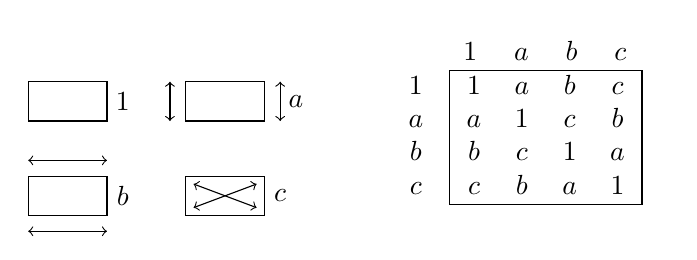
\begin{tikzpicture}
        \draw[draw=black] (0,0) rectangle ++(1,0.5);
        \node at (1.2, 0.25) {1};
        
        \draw[draw=black] (2,0) rectangle ++(1,0.5);
        \draw[<->] (1.8, 0) -- (1.8, 0.5);
        \draw[<->] (3.2, 0) -- (3.2, 0.5);
        \node at (3.4, 0.25) {$a$};
        
        \draw[draw=black] (0,-1.2) rectangle ++(1,0.5);
        \draw[<->] (0, -0.5) -- (1, -0.5);
        \draw[<->] (0, -1.4) -- (1, -1.4);
        \node at (1.2, -0.95) {$b$};
        
        \draw[draw=black] (2,-1.2) rectangle ++(1,0.5);
        \draw[<->] (2.1, -1.1) -- (2.9, -0.8);
        \draw[<->] (2.1, -0.8) -- (2.9, -1.1);
        \node at (3.2, -0.95) {$c$};
        
        \node at (6,0) {\begin{tabular}{c c}
         & \, \, \, \, 1 \, \,  $a$ \, \, $b$ \, \, $c$ \\
         & \begin{tabular}{c}
              1  \\ $a$ \\ $b$ \\ $c$
         \end{tabular}
         \begin{tabular}{|c c c c|}
        \hline 
         1 & $a$ & $b$ & $c$ \\
         $a$ & 1 & $c$ & $b$ \\
         $b$ & $c$ & 1 & $a$ \\
         $c$ & $b$ & $a$ & 1 \\ \hline
    \end{tabular} \\
    \end{tabular} };
    \end{tikzpicture}\]
    We get the graph: 
    \[ 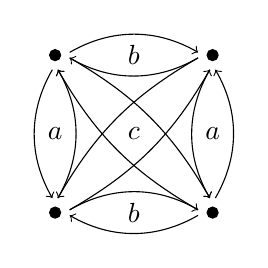
\begin{tikzpicture}
        \filldraw [black] (1, 1) circle (2pt);
        \filldraw [black] (1, -1) circle (2pt);
        \filldraw [black] (-1, 1) circle (2pt);
        \filldraw [black] (-1, -1) circle (2pt);
        
        \node (A) at (-1,1) {};
        \node (B) at (1,1) {};
        \node (C) at (1, -1) {};
        \node (D) at (-1, -1) {};
        
        \draw[->, shorten >=2pt,shorten <=2pt] (A.south) to [out=240, in=120] (D.north);
        \draw[<-, shorten >=2pt,shorten <=2pt] (A.south) to [out=300, in=60] (D.north);
        \draw[->, shorten >=2pt,shorten <=2pt] (B.south) to [out=240, in=120] (C.north);
        \draw[<-, shorten >=2pt,shorten <=2pt] (B.south) to [out=300, in=60] (C.north);
        
        \draw[->, shorten >=2pt,shorten <=2pt] (A.east) to [out=30, in=150] (B.west);
        \draw[<-, shorten >=2pt,shorten <=2pt] (A.east) to [out=330, in=210] (B.west);
        \draw[->, shorten >=2pt,shorten <=2pt] (D.east) to [out=30, in=150] (C.west);
        \draw[<-, shorten >=2pt,shorten <=2pt] (D.east) to [out=330, in=210] (C.west);
        
        \draw[->, shorten >=2pt,shorten <=2pt] (A.east) to [out=330, in=120] (C.north);
        \draw[<-, shorten >=2pt, shorten <=2pt] (A.south) [out=300, in=150] to (C.west);
        \draw[->, shorten >=2pt,shorten <=2pt] (B.west) [out=210, in=60] to (D.north) ;
        \draw[<-, shorten >=2pt,shorten <=2pt] (B.south) [out=240, in=30] to (D.east) ;
        
        \node at (-1,0) {$a$};
        \node at (1,0) {$a$};
        \node at (0, -1) {$b$};
        \node at (0, 1) {$b$};
        \node at (0,0) {$c$};
    \end{tikzpicture}\]
\end{example}

\noindent
Cayley graph: Point for each $g \in G$ Draw a line from $g$ to $h$ with $gf=h$. \\

\noindent
Goal of Group theory
\begin{enumerate}
    \item Classify all groups 
    \begin{itemize}
        \item Hard but can do special cases: Groups of order 60, finite subgroups of rotations in $\bR^3$, all finite simple groups, symmetries of crystals 
    \end{itemize}
    \item Given a group $G$, classify all ways $G$ can act on something (called a representation of $G$)
    \begin{itemize}
        \item Permutation representation : $G$ acts on a set $S$
        \item Linear representation : $G$ acts on a vector space 
    \end{itemize}
\end{enumerate}

\begin{example}
    Poncaire group = symmetries of space time \\
    elementary particle: space of states = vector space acted on by $G$ = linear group of $G$
\end{example}

\subsection{Review of homomorphisms, isomorphims} 

\begin{definition}
    A homomorphism is a map $f : G \to H$ that preserves structure \\
    eg. $f(gh)=f(g)f(h)$, $f(1)=1$, $f(g^{-1}) = f(g)^{-1}$ 
\end{definition}
Note: last two properties can be derived from the first. 

\begin{example}
    $\exp(x)=e^x$ : $(\bR, +) \to (\bR, \times)$ \\
    $\exp(x+y)=\exp(x)\exp(y)$, $\exp(0)=1$, $\exp(-x)=\exp(x)^{-1}$
\end{example}

\begin{definition}
    The kernel of a homomorphism $f$ is the set of elements with image the identity. 
\end{definition}

\begin{example}
    $\bR \to $ rotation is the plane by $\theta \mapsto$ rotation by angle $\theta$. \\
    nontrivial kernel : multiples of $2 \pi$. \\
    We get the short exact sequence: $0 \to 2\pi\bZ \to \bR \to \text{rotations} \to 0$ 
\end{example}

\begin{definition}
    A sequence of homomorphisms $A \to B \to C$ is exact if Image $A \to B$ = Kernel $B \to C$
\end{definition}
$0 \to A \to B$ means $A \to B$ is injective \\
$A \to B \to 0$ means $A \to B$ is surjective 

\begin{definition}
    $f : A \to B$ is an isomorphim if it is a homomorphism with an inverse. We say $A,B$ are isomorphic. ``basically the same''
\end{definition}

\begin{example}
    $2 \pi \bZ$ is isomorphic to $\bZ$.
\end{example}

\begin{example}
    $\bZ/4\bZ$, integers mod 4 with addition: $\{0, 1, 2, 3\}$ and $(\bZ/5\bZ)^{\times}$, under multiplcation: $\{1, 2, 3, 4 \}$ are isomorphic. \\
    We map $0 \to 1=2^0$, $1 \to 2 = 2^1$, $2 \to 4=2^2$, $3 \to 3= 2^3$    eg. $x \mapsto 2^x$
\end{example}

\subsection{Classify all finite groups up to isomorphim}

\begin{definition}
    The order of a group $G$ = number of elements in $G$
\end{definition}

\noindent
\textbf{Order 1}: $e \times e = e$ \quad 1 group - trivial group

\noindent 
\textbf{Order 2}: 1 group - $e,f$ with $f^2=e$ $\cong \bZ/2\bZ$ 

\noindent
\textbf{Order $p$ for $p$ prime}: only one group $\bZ/p\bZ$ (integers modulo $p$)

\begin{definition}
    For $g \in G$ the order of $g$ is the smallest $ n \ge 1$ with $g^n=1$
\end{definition}

\begin{theorem}[Lagrange's Theorem]
    If $g \in G$, the roder of $g$ divides the order of $G$. 
\end{theorem}

\begin{example}
    Suppose $|G|=p$, ($p$ prime). Pick $g \in G$ with $g \neq e$. Order of $g$ divides $|G|=p$ so is either 1 or $p$. Can't be one since $g \neq e$. So elemenets of $G$ $1, g, \ldots, g^{p-1}$ are all distinct since $g^p=1$, $g^x \neq 1$ for $0 \le x < p$ and if $g^i = g^j, g^{i-j}=1$. Thus, these must be all elements of $G$. 
\end{example}

\noindent
\textbf{Order 4}: 
\begin{itemize}
    \item Ex : $\bZ/4\bZ$, symmetries of rectangle, $(\bZ/5\bZ)^{\times}$, $(\bZ/8\bZ)^{\times}$, symmetries of (Insert Figure)
    \item only 2 groups of order 4
\end{itemize}